\documentclass[a4paper]{article}
\usepackage[utf8]{inputenc}




\title{Leggi di Newton e urti centrali elastici e anelastici\\ analisi dati}
\author{Ali Matteo,\\Broggi Diana, Cantarini Giulia}
\date{ }

\usepackage{tabularx}
\usepackage{natbib}
%\usepackage[demo]{graphicx}
\usepackage{graphicx}

%\usepackage[margin=1.0in]{geometry}

\usepackage{tikz}

\usepackage{caption}
%\usepackage[font=small,labelfont=bf]{caption}

\usepackage{subcaption}
   

\usepackage{amsmath, amsthm}

\usepackage{mathrsfs}

\usepackage{pgfplots}
%\usepackage{ragged2e}



%\pgfplotsset{width=4cm,compat=1.9}

\theoremstyle{definition}
\newtheorem{rich}{richiamo matematico}[section]





%roba che crea comando per centrare immagine dentro immagine piu grande
%https://tex.stackexchange.com/a/308286
\newlength{\imagew}
\newlength{\imageh}
\newlength{\legendw}
\newlength{\legendh}
\newlength{\legendx}
\newlength{\legendy}
\newcommand{\graphicswithlegend}[6]{
	\setlength{\imagew}{#1}
	\settoheight{\imageh}{\includegraphics[width=\imagew]{#2}}
	
	\setlength{\legendw}{#3\imagew}
	\settoheight{\legendh}{\includegraphics[width=\legendw]{#4}}
	
	\setlength{\legendx}{\imagew}
	\addtolength{\legendx}{-\legendw}
	\addtolength{\legendx}{-#5\imagew}
	
	\setlength{\legendy}{\imageh}
	\addtolength{\legendy}{-\legendh}
	\addtolength{\legendy}{-#6\imageh}
	
	\includegraphics[width=\imagew]{#2}%
	\llap{
		\hspace{-\the\legendx}
		\raisebox{\legendy}{\includegraphics[width=\legendw]{#4}}
		\hspace{\the\legendx}
	}
}



\begin{document}
	\pagenumbering{arabic}
	\maketitle
\subsection*{urti tra due carrelli}

\begin{figure}[!ht]
		\captionsetup{labelformat=empty}
	\caption{Grafico \(v_{(t)}\) run 1 urto elastico}
	\makebox[1 \textwidth][c]{       %centering table
		\resizebox{0.90 \textwidth}{!}{   %resize table
			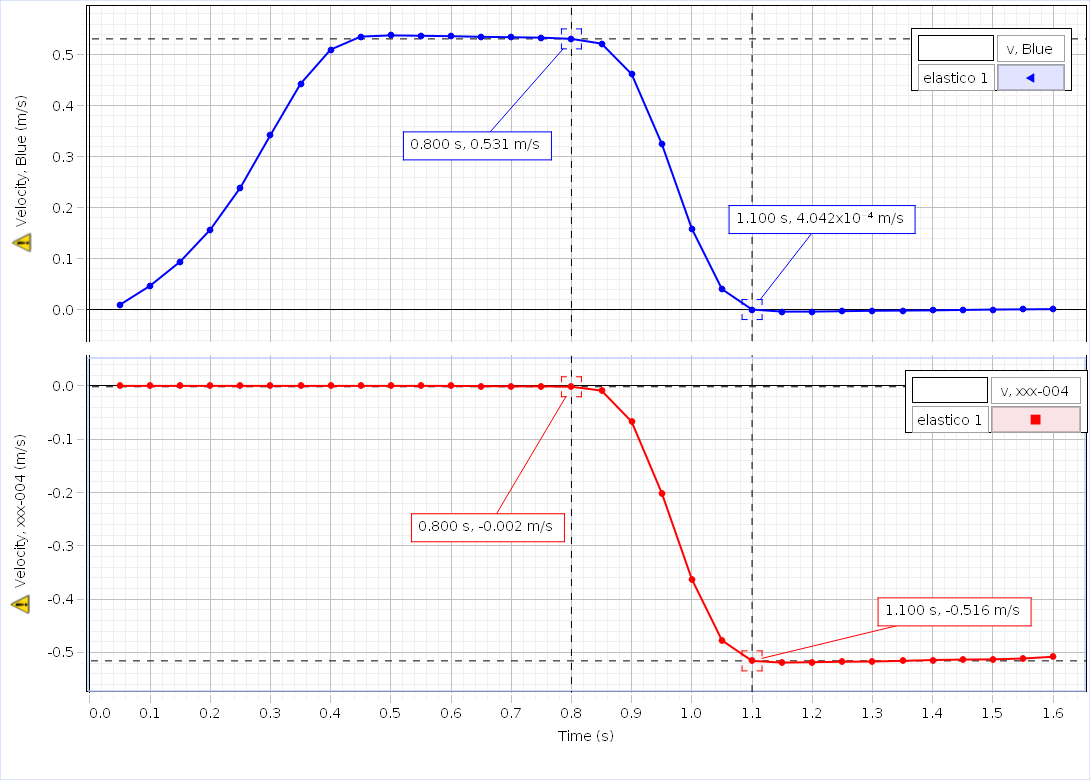
\includegraphics{capstone_data/elastico_vel.png}
		} %close resize
	} %close centering
	
\end{figure}
\[v_{f R} = v_{i B} \frac{2 m_{B}}{m_{R}+m_{B}}\]
\begin{minipage}[c]{0.5\textwidth}
		\captionsetup{labelformat=empty}
			\captionof{table}{carrello blu \(v_{f} = 0\)}
	\centering
	\begin{tabular}{||cc||}
		\hline
		\hline
		run &  \(v_{i}\) (m/s)\\
		\hline
		1: & 0.531  \\ 
		2: & 0.474\\
		3: & 0.380\\
		4: & 0.558\\
		5: & 0.642\\
		\hline
		\hline
	\end{tabular}

\end{minipage}
\begin{minipage}[c]{0.5\textwidth}
			\captionsetup{labelformat=empty}
				\captionof{table}{carrello rosso \(v_{i} = 0\)}
	\centering
	\begin{tabular}{||ccc||}
		\hline
		\hline
		run &  \(v_{fosservata}\) (m/s) & \(v_{fattesa}\) (m/s)\\
		\hline
		1: & 0.516 & 0.528 \\
		2: & 0.469& 0.472\\
		3: & 0.368& 0.378\\
		4: & 0.544& 0.555\\
		5: & 0.618& 0.639\\
		\hline
		\hline
	\end{tabular}
\end{minipage}

\[v_{f R} = v_{i B} \frac{2 (0.270 Kg)}{0.543 Kg}\]

\[t = \frac{ \left |\bar{v_{oss}}  - \bar{v_{att}} \right |}{\sqrt{\sigma_{vosservata}^{2}+ \sigma_{vattesa}^{2}}} = 0.19\]
\noindent \(\rightarrow\) la probabilità che la differenza sia dovuta solo ad errori casuali è del 85\(\%\).\\\\

\begin{figure}[!ht]
	\captionsetup{labelformat=empty}
	\caption{Grafico \(v_{(t)}\) run 1 urto elastico (con carrello blu caricato con 500g)}
	\makebox[1 \textwidth][c]{       %centering table
		\resizebox{0.90 \textwidth}{!}{   %resize table
			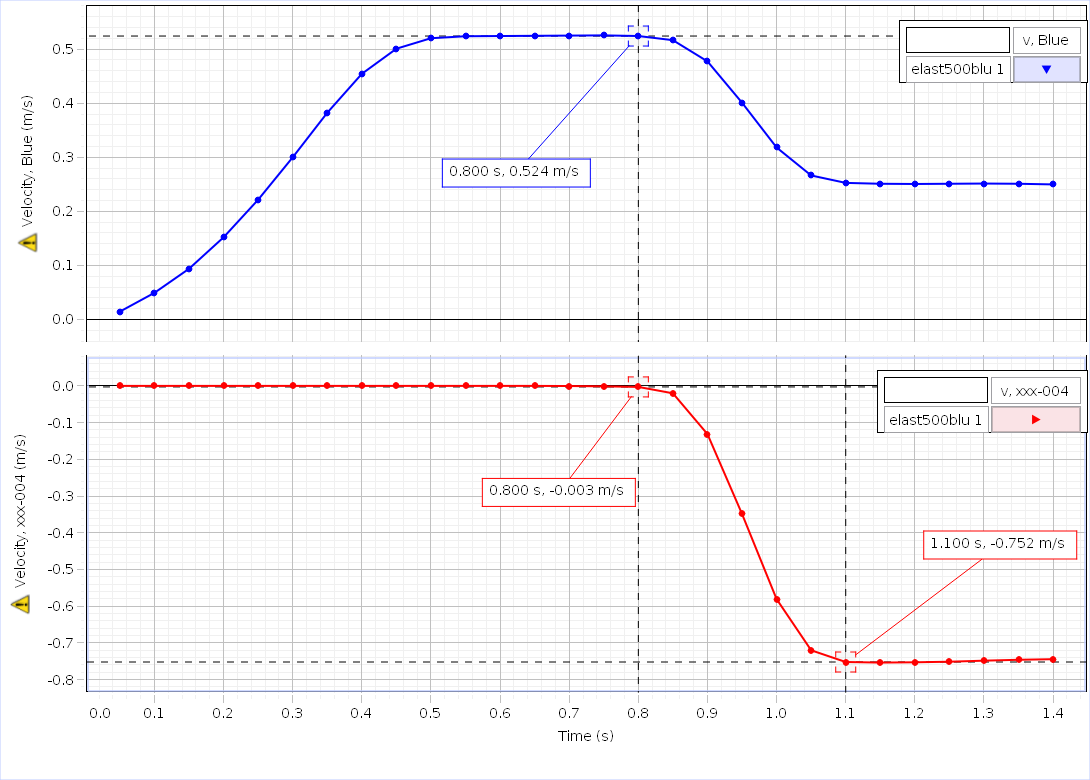
\includegraphics{capstone_data/elastico_500_blu_vel.png}
		} %close resize
	} %close centering
	
\end{figure}

\begin{minipage}[c]{0.5\textwidth}
	\captionsetup{labelformat=empty}
	\captionof{table}{carrello blu \(v_{f} = 0\)}
	\centering
	\begin{tabular}{||cc||}
		\hline
		\hline
		run &  \(v_{i}\) (m/s)\\
		\hline
		1: & 0.524   \\ 
		2: & 0.400\\
		3: & 0.376\\
		4: & 0.612\\
		5: & 0.829\\
		\hline
		\hline
	\end{tabular}
	
\end{minipage}
\begin{minipage}[c]{0.5\textwidth}
	\captionsetup{labelformat=empty}
	\captionof{table}{carrello rosso \(v_{i} = 0\)}
	\centering
	\begin{tabular}{||ccc||}
		\hline
		\hline
		run &  \(v_{fosservata}\) (m/s) & \(v_{fattesa}\) (m/s)\\
		\hline
		1: & 0.752 & 0.775 \\
		2: &0.576& 0.592\\
		3: &0.543& 0.556\\
		4: & 0.881& 0.906\\
		5: &0.808& 0.828\\
		\hline
		\hline
	\end{tabular}
\end{minipage}

\[v_{f R} = v_{i B} \frac{2 (0.777 Kg)}{1.050 Kg}\]

\[t = \frac{ \left |\bar{v_{oss}}  - \bar{v_{att}} \right |}{\sqrt{\sigma_{vosservata}^{2}+ \sigma_{vattesa}^{2}}} = 0.2 \]
\noindent \(\rightarrow\) la probabilità che la differenza sia dovuta solo ad errori casuali è del 84\(\%\).
\begin{figure}[!ht]
	\captionsetup{labelformat=empty}
	\caption{Grafico \(v_{(t)}\) run 1 urto elastico (con carrello rosso caricato con 500g)}
	\makebox[1 \textwidth][c]{       %centering table
		\resizebox{0.90 \textwidth}{!}{   %resize table
			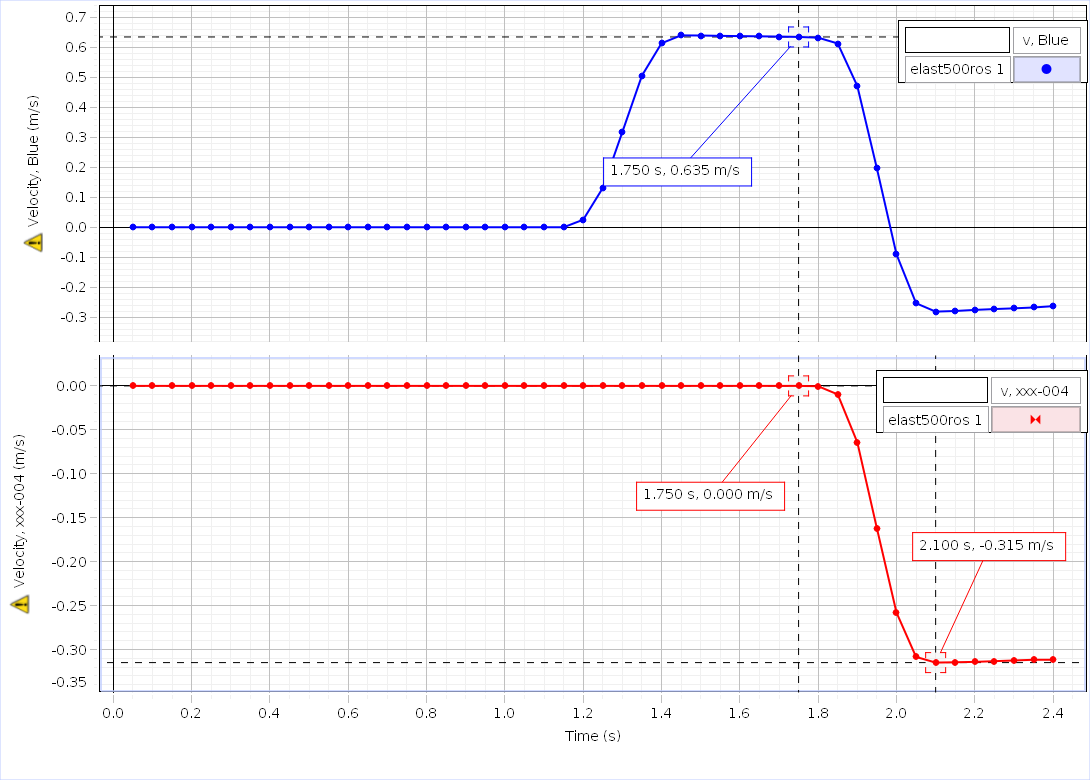
\includegraphics{capstone_data/elastico_500_rosso_vel.png}
		} %close resize
	} %close centering
	
\end{figure}

\begin{minipage}[c]{0.5\textwidth}
	\captionsetup{labelformat=empty}
	\captionof{table}{carrello blu \(v_{f} = 0\)}
	\centering
	\begin{tabular}{||cc||}
		\hline
		\hline
		run &  \(v_{i}\) (m/s)\\
		\hline
		1: &0.635  \\ 
		2: &0.640 \\
		3: &0.405 \\
		4: &0.547\\
		5: &0.528 \\
		\hline
		\hline
	\end{tabular}
	
\end{minipage}
\begin{minipage}[c]{0.5\textwidth}
	\captionsetup{labelformat=empty}
	\captionof{table}{carrello rosso \(v_{i} = 0\)}
	\centering
	\begin{tabular}{||ccc||}
		\hline
		\hline
		run &  \(v_{fosservata}\) (m/s) & \(v_{fattesa}\) (m/s)\\
		\hline
		1: &0.315  & 0.327\\
		2: &0.320 &0.330\\
		3: &0.201&0.209\\
		4: &0.277 &0.282\\
		5: & 0.264&0.272\\
		\hline
		\hline
	\end{tabular}
\end{minipage}

\[v_{f R} = v_{i B} \frac{2 (0.270 Kg)}{1.050 Kg}\]

\[t = \frac{ \left |\bar{v_{oss}}  - \bar{v_{att}} \right |}{\sqrt{\sigma_{vosservata}^{2}+ \sigma_{vattesa}^{2}}} = 0.28 \]
\noindent \(\rightarrow\) la probabilità che la differenza sia dovuta solo ad errori casuali è del 78\(\%\).\\\\\\\\\\\\\\\\\\\\\\\\\\


\begin{figure}[!htbp]
	\captionsetup{labelformat=empty}
	\caption{urto anaelastico (carrelli vuoti, \(v_{iR} = 0\))}
	\makebox[1 \textwidth][c]{       %centering table
		\resizebox{1.70 \textwidth}{!}{
			\begin{subfigure}{0.9\textwidth}
				\caption{quantità di moto}
				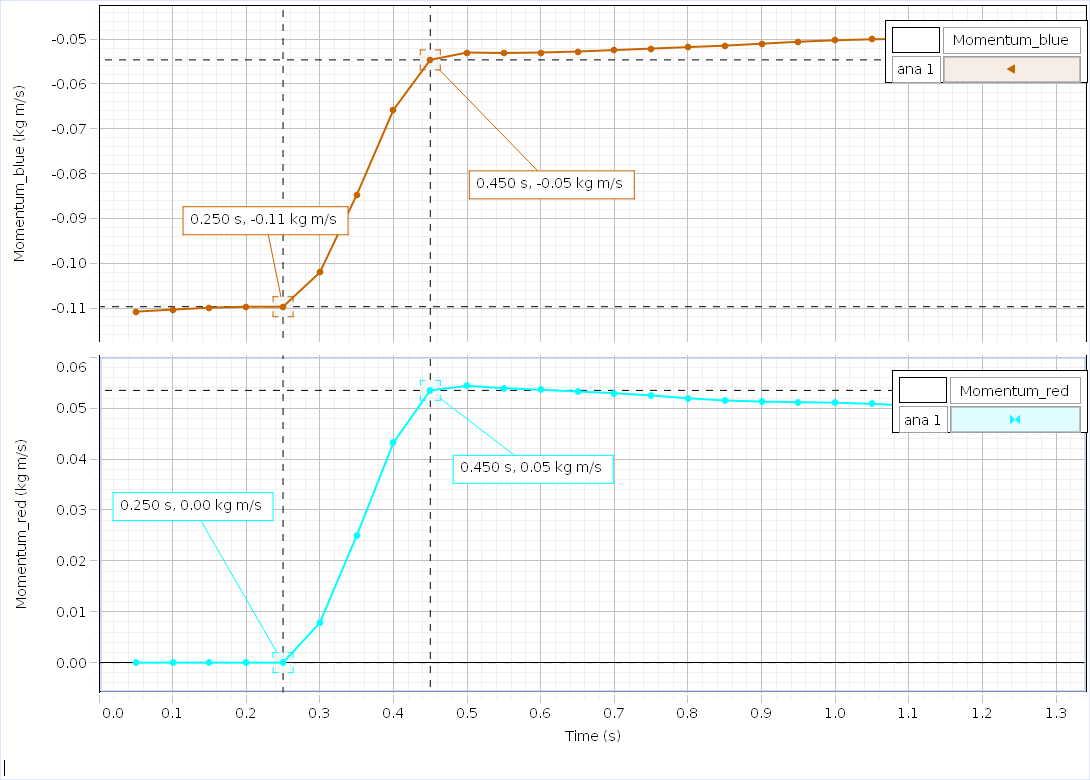
\includegraphics[scale=0.45]{capstone_data/anaelastico_momento.png}
			\end{subfigure}%
			
			\begin{subfigure}{0.9\textwidth}
				\caption{energia cinetica}
				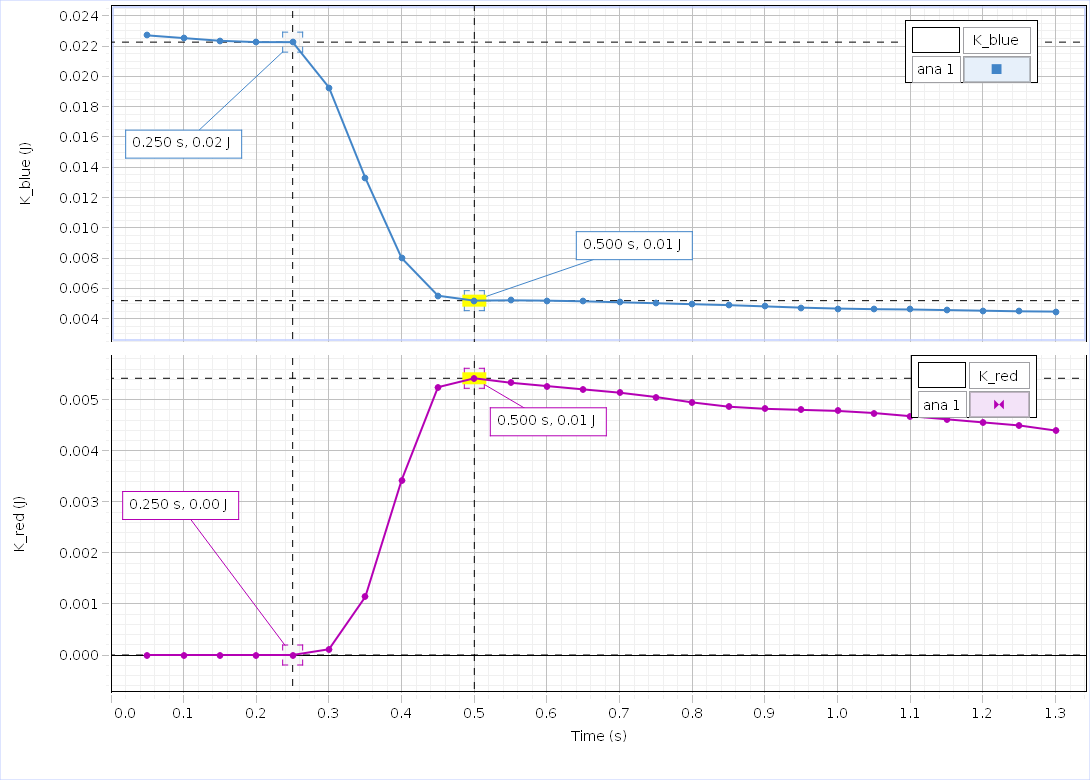
\includegraphics[scale=0.45]{capstone_data/anaelastico_Ec.png}
			\end{subfigure}%
		}
	}
\end{figure}


		
	\begin{figure}[!htbp]
				\captionsetup{labelformat=empty}
		\caption{Tabella variazione della quantità di moto}
		\makebox[1 \textwidth][c]{ 
			\begin{tabular}{||ccc|c||}
				\hline
				\hline
				run &  \(\Delta p\)  carrello blu (Kg m/s) & \(\Delta p\)  carrello rosso (Kg m/s)& \(\Delta p\)  totale (Kg m/s)\\
				\hline
				1: &0.055-0.110 = -0.055 & 0.054-0 =  0.054 & -0.001\\ 
				2: &0.060-0.121 = -0.061& 0.061-0 =   0.061& 0\\
				3: &0.060-0.123 = -0.063 & 0.060-0 = 0.060 & -0.003\\
				4: &0.052-0.108 = -0.056 & 0.053-0 = 0.053 & -0.003\\
				5: &0.072-0.148 = -0.076& 0.073-0 = 0.073& -0.003\\
				\hline
				\hline
			\end{tabular}
		} %close centering
	\end{figure}

	\[t = \frac{\left | \bar{\Delta p} - 0\right |}{\sigma_{\Delta p}} = 3.3\]
	\noindent \(\rightarrow\) la probabilità che la discrepanza con \(\Delta p = 0\) sia dovuto solo ad errori casuali è del 0.1 \(\%\), risultato non accettabile.
\begin{figure}[!htbp]
	\captionsetup{labelformat=empty}
	\caption{Tabella variazione della energia cinetica}
	\makebox[1 \textwidth][c]{ 
		\begin{tabular}{||ccc|c||}
			\hline
			\hline
			run &  \(\Delta Ec\)  carrello blu (J) & \(\Delta Ec\)  carrello rosso (J) & \(\Delta Ec\)  totale (J)\\
			\hline
			1: & 0.005-0.022 = -0.017&0.0054-0 = 0.0054 & -0.012 \\ 
			2: &0.006-0.027 = -0.021 & 0.0067-0 = 0.0067& -0.014\\
			3: &0.007-0.028 = -0.021&0.007-0 = 0.007 & -0.014\\
			4: &0.0049-0.0214 = -0.017 & 0.005-0 = 0.005& -0.012\\
			5: &0.010-0.040 = -0.030 & 0.010-0 = 0.010 & -0.02 \\
			\hline
			\hline
		\end{tabular}
	} %close centering
\end{figure}

\begin{figure}[!htbp]
	\captionsetup{labelformat=empty}
	\caption{urto anaelastico (carrello blu caricato con 500g, \(v_{iR} = 0\))}
	\makebox[1 \textwidth][c]{       %centering table
		\resizebox{1.70 \textwidth}{!}{
			\begin{subfigure}{0.9\textwidth}
				\caption{quantità di moto}
				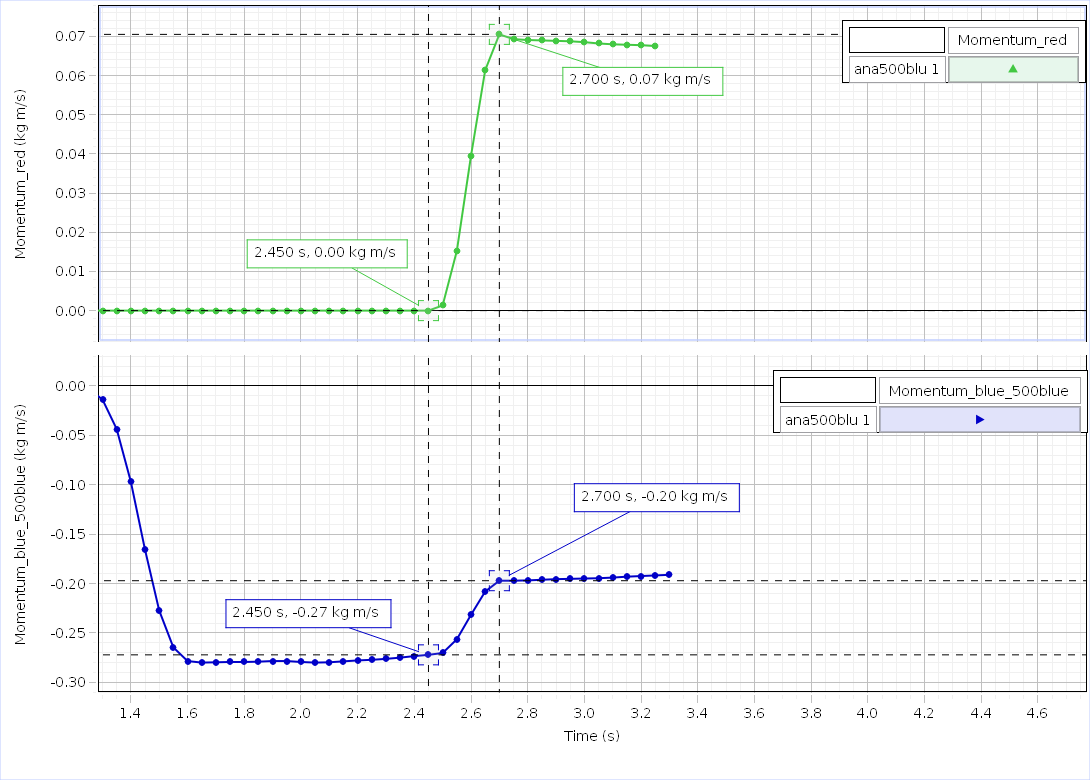
\includegraphics[scale=0.45]{capstone_data/anaelastico_500_blu_momento.png}
			\end{subfigure}%
			
			\begin{subfigure}{0.9\textwidth}
				\caption{energia cinetica}
				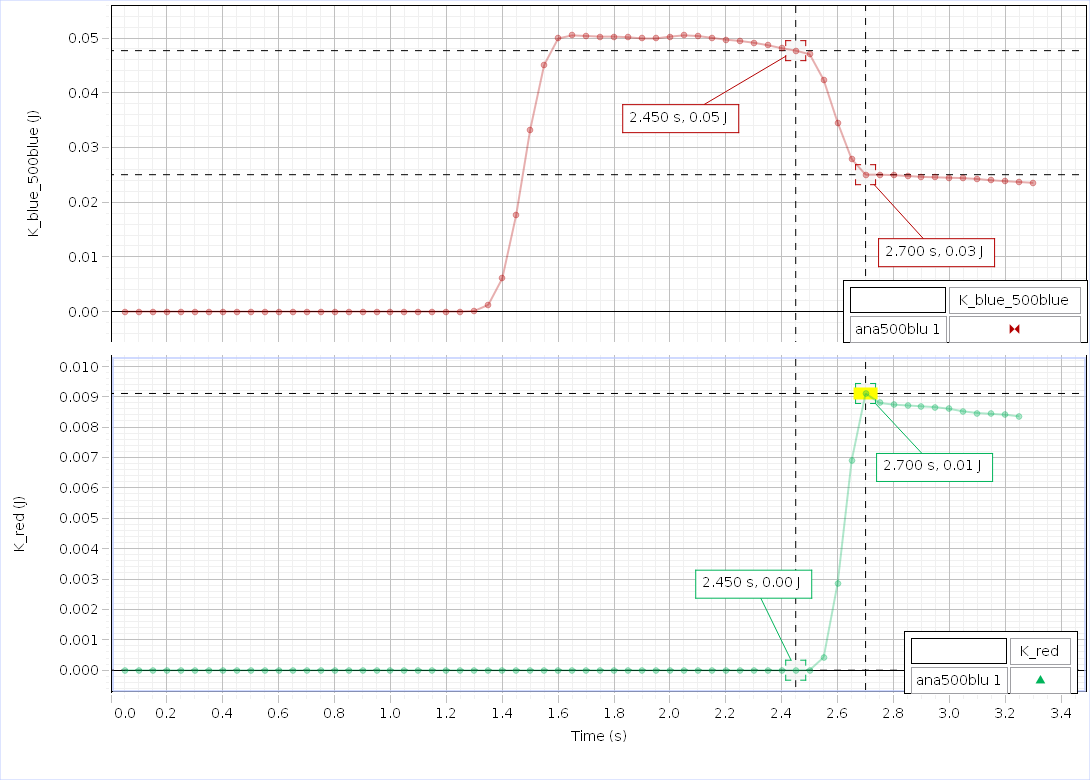
\includegraphics[scale=0.45]{capstone_data/anaelastico_500_blu_Ec.png}
			\end{subfigure}%
		}
	}
\end{figure}



\begin{figure}[!htbp]
	\captionsetup{labelformat=empty}
	\caption{Tabella variazione della quantità di moto}
	\makebox[1 \textwidth][c]{ 
		\begin{tabular}{||ccc|c||}
			\hline
			\hline
			run &  \(\Delta p\)  carrello blu (Kg m/s) & \(\Delta p\)  carrello rosso (Kg m/s)& \(\Delta p\)  totale (Kg m/s)\\
			\hline
			1: &0.200-0.272 = -0.072& 0.071-0 = 0.071& -0.001\\
			2: &0.328-0.456 = -0.128 &0.114-0 = 0.114& -0.014\\
			3: &0.213-0.295 = -0.082& 0.076-0 = 0.076&-0.006\\
			4: &0.227-0.311 = -0.084 & 0.0813-0 = 0.081& -0.003\\
			5: &0.233-0.317 = -0.084& 0.082-0 = 0.082 &-0.002\\
			\hline
			\hline
		\end{tabular}
	} %close centering
\end{figure}

	\[t = \frac{\left | \bar{\Delta p} - 0\right |}{\sigma_{\Delta p}} = 2.2\]
\noindent \(\rightarrow\) la probabilità che la discrepanza con \(\Delta p = 0\) sia dovuto solo ad errori casuali è del 3\(\%\), risultato non accettabile.


\begin{figure}[!htbp]
	\captionsetup{labelformat=empty}
	\caption{Tabella variazione della energia cinetica}
	\makebox[1 \textwidth][c]{ 
		\begin{tabular}{||ccc|c||}
			\hline
			\hline
			run &  \(\Delta Ec\)  carrello blu (J) & \(\Delta Ec\)  carrello rosso (J) & \(\Delta Ec\)  totale (J)\\
			\hline
			1: & 0.025-0.048 = -0.023 &0.009-0 = 0.009 & -0.014\\
			2: & 0.069-0.134 = -0.065& 0.024-0 = 0.024 & 0.041\\
			3: &0.029-0.056 = -0.027& 0.011-0 = 0.011 & -0.016\\
			4: & 0.033-0.062 = -0.029& 0.012-0 = 0.012& -0.017\\
			5:&0.035-0.065 = -0.030 & 0.012-0 = 0.012 & -0.018\\
			\hline
			\hline
		\end{tabular}
	} %close centering
\end{figure}

\begin{figure}[!htbp]
	\captionsetup{labelformat=empty}
	\caption{urto anaelastico (carrello rosso caricato con 500g, \(v_{iR} = 0\))}
	\makebox[1 \textwidth][c]{       %centering table
		\resizebox{1.70 \textwidth}{!}{
			\begin{subfigure}{0.9\textwidth}
				\caption{quantità di moto}
				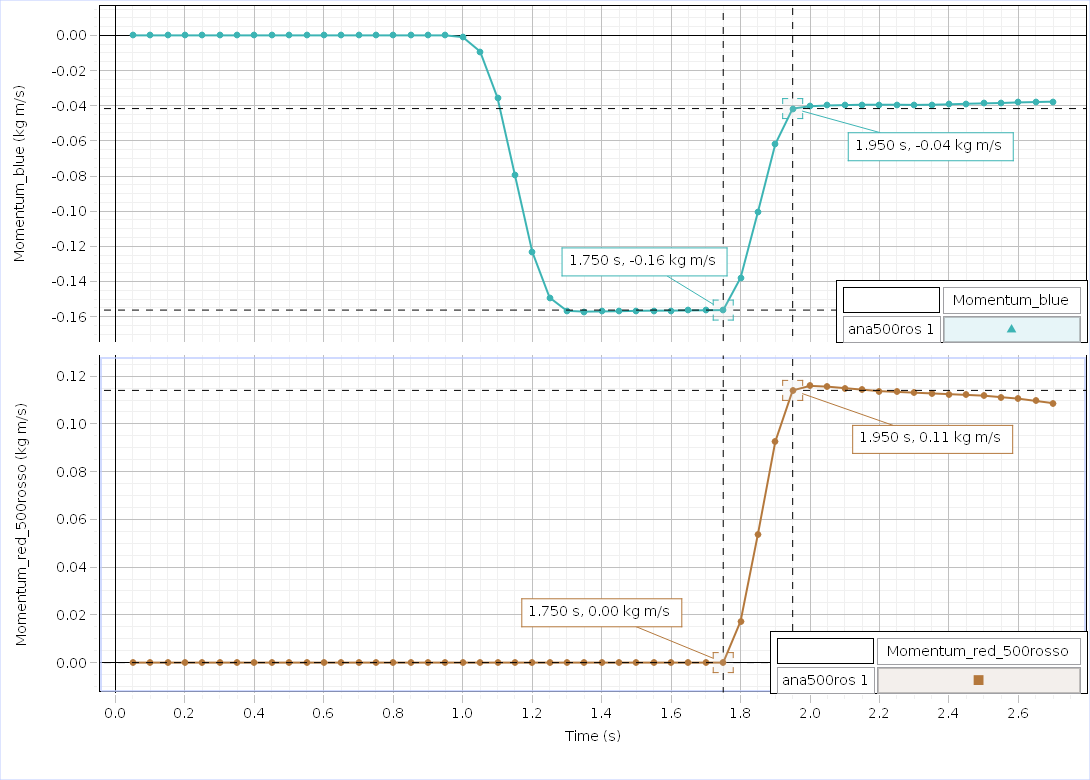
\includegraphics[scale=0.45]{capstone_data/anaelastico_500_rosso_momento.png}
			\end{subfigure}%
			
			\begin{subfigure}{0.9\textwidth}
				\caption{energia cinetica}
				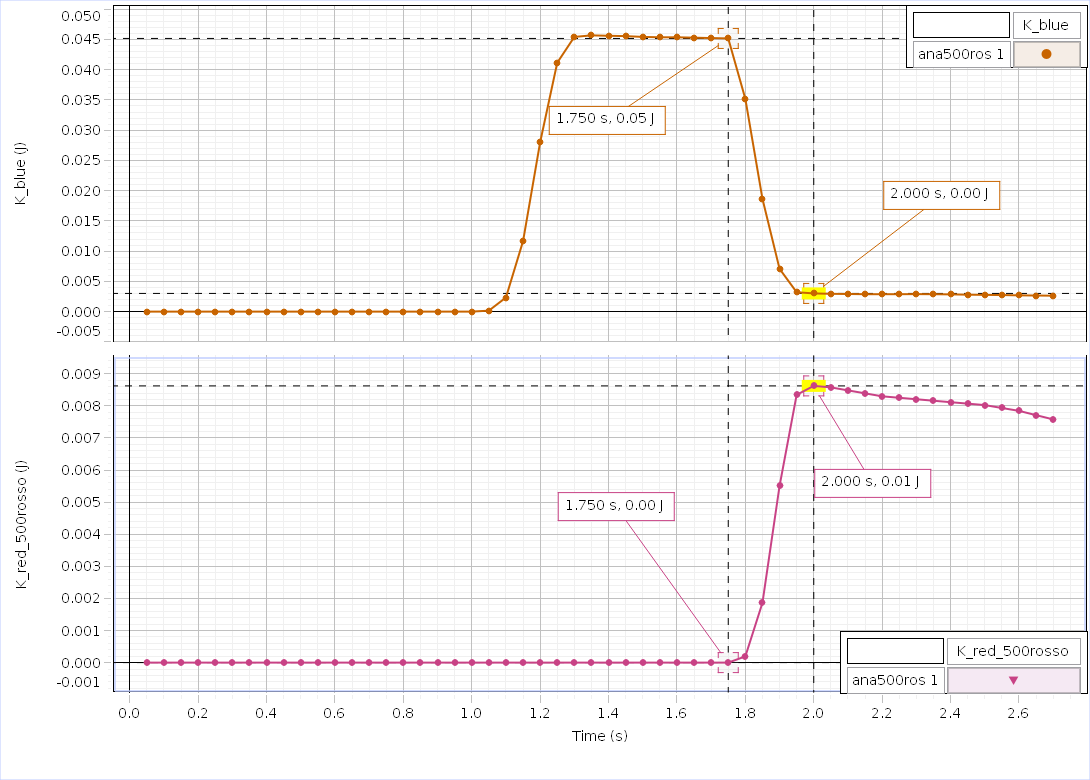
\includegraphics[scale=0.45]{capstone_data/anaelastico_500_rosso_Ec.png}
			\end{subfigure}%
		}
	}
\end{figure}



\begin{figure}[!htbp]
	\captionsetup{labelformat=empty}
	\caption{Tabella variazione della quantità di moto}
	\makebox[1 \textwidth][c]{ 
		\begin{tabular}{||ccc|c||}
			\hline
			\hline
			run &  \(\Delta p\)  carrello blu (Kg m/s) & \(\Delta p\)  carrello rosso (Kg m/s)& \(\Delta p\)  totale (Kg m/s)\\
			\hline
			1: & 0.040-0.156 = -0.116&0.116-0= 0.116 & 0\\
			2: &0.044-0.169 = -0.125& 0.126-0 = 0.126 & 0.001\\
			3: &0.049-0.188 = -0.139& 0.140-0 = 0.140 & 0.001\\
			4: & 0.039-0.162 = -0.123& 0.122-0 = 0.122 &-0.001\\
			5: & 0.050+0.202 = -0.152& 0.151- 0 = 0.151 &-0.001\\
			\hline
			\hline
		\end{tabular}
	} %close centering
\end{figure}

	\[t = \frac{\left | \bar{\Delta p} - 0\right |}{\sigma_{\Delta p}} = 0\]
\noindent \(\rightarrow\) la probabilità che la discrepanza con \(\Delta p = 0\) nei diversi run sia dovuto solo ad errori casuali è del 100\(\%\).

\begin{figure}[!htbp]
	\captionsetup{labelformat=empty}
	\caption{Tabella variazione della energia cinetica}
	\makebox[1 \textwidth][c]{ 
		\begin{tabular}{||ccc|c||}
			\hline
			\hline
			run &  \(\Delta Ec\)  carrello blu (J) & \(\Delta Ec\)  carrello rosso (J) & \(\Delta Ec\)  totale (J)\\
			\hline
			1:& 0.003-0.045 = -0.042& 0.009- 0 = 0.009 & -0.033\\
			2: &0.004-0.053 = -0.049 & 0.010-0 = 0.010 &-0.039\\
			3: &0.004-0.065 = -0.061 &0.013-0 = 0.013 & -0.048\\
			4: & 0.003-0.048 = -0.045& 0.010-0 = 0.010 & -0.035\\
			5: & 0.005-0.075 = -0.070&0.015-0 = 0.015 & -0.055\\
			\hline
			\hline
		\end{tabular}
	} %close centering
\end{figure}

\subsection*{calcolo del coefficiente di attrito}

\begin{figure}[!ht]
	\captionsetup{labelformat=empty}
	\caption{Grafico \(F_{(x)}\) con un libro davanti al carrello sottoposto a tensione}
	\makebox[1 \textwidth][c]{       %centering table
		\resizebox{0.90 \textwidth}{!}{   %resize table
			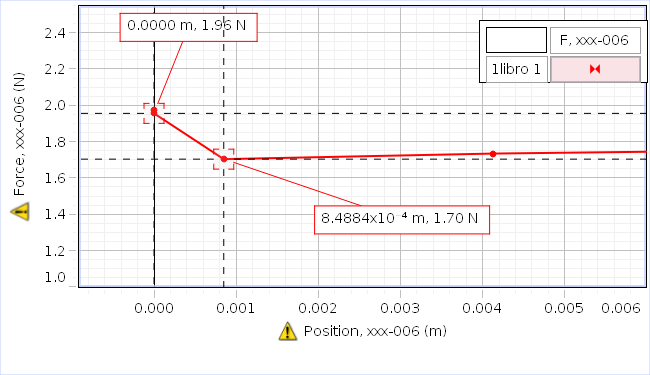
\includegraphics{capstone_data/1libro.png}
		} %close resize
	} %close centering
	
\end{figure}

\begin{figure}[!htbp]
	\captionsetup{labelformat=empty}
	\caption{1 Libro, \(m_{libro} = 0.482 Kg\)}
	\makebox[1 \textwidth][c]{ 
		\begin{tabular}{ccc}
			\hline
			\hline
			run & \(F_{a}\) (N)& \(\mu\)\\
			\hline
			1: & 0.26 & 0.055\\ 
			2: & 0.27 & 0.057\\
			3: &0.29 & 0.06\\
			4: &0.22 & 0.005\\
			5: & 0.13 & 0.027\\
			\hline
			\hline
		\end{tabular}
	} %close centering
\end{figure}

\begin{figure}[!ht]
	\captionsetup{labelformat=empty}
	\caption{Grafico \(F_{(x)}\) con due libri davanti al carrello sottoposto a tensione}
	\makebox[1 \textwidth][c]{       %centering table
		\resizebox{0.90 \textwidth}{!}{   %resize table
			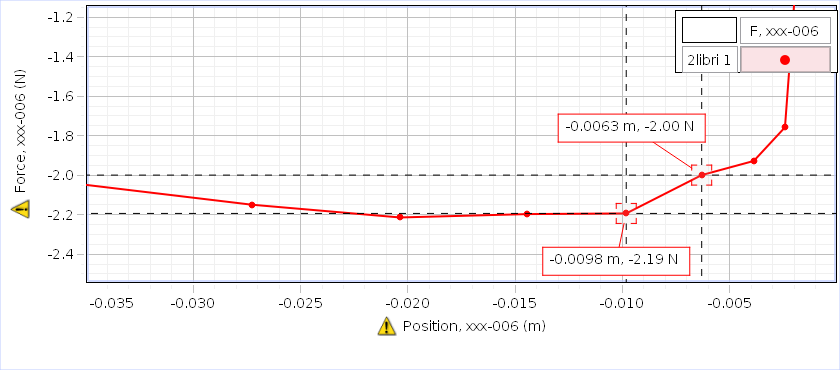
\includegraphics{capstone_data/2libri.png}
		} %close resize
	} %close centering
	
\end{figure}

\begin{figure}[!htbp]
	\captionsetup{labelformat=empty}
	\caption{2 Libri, \(m_{libri tot} = 0.798 Kg\)}
	\makebox[1 \textwidth][c]{ 
		\begin{tabular}{ccc}
			\hline
			\hline
			run & \(F_{a}\) (N)& \(\mu\)\\
			\hline
			1: & 0.19 & 0.024\\ 
			2: & 0.19 & 0.024\\
			3: &0.04 & 0.005\\
			4: &0.10 & 0.013\\
			5: & 0.25 & 0.032\\
			\hline
			\hline
		\end{tabular}
	} %close centering
\end{figure}


\begin{figure}[!htbp]
	\captionsetup{labelformat=empty}
	\caption{urto anaelastico (carrello rosso caricato con 500g, \(v_{iR} = 0\))}
	\makebox[1 \textwidth][c]{       %centering table
		\resizebox{1.70 \textwidth}{!}{
			\begin{subfigure}{0.9\textwidth}
				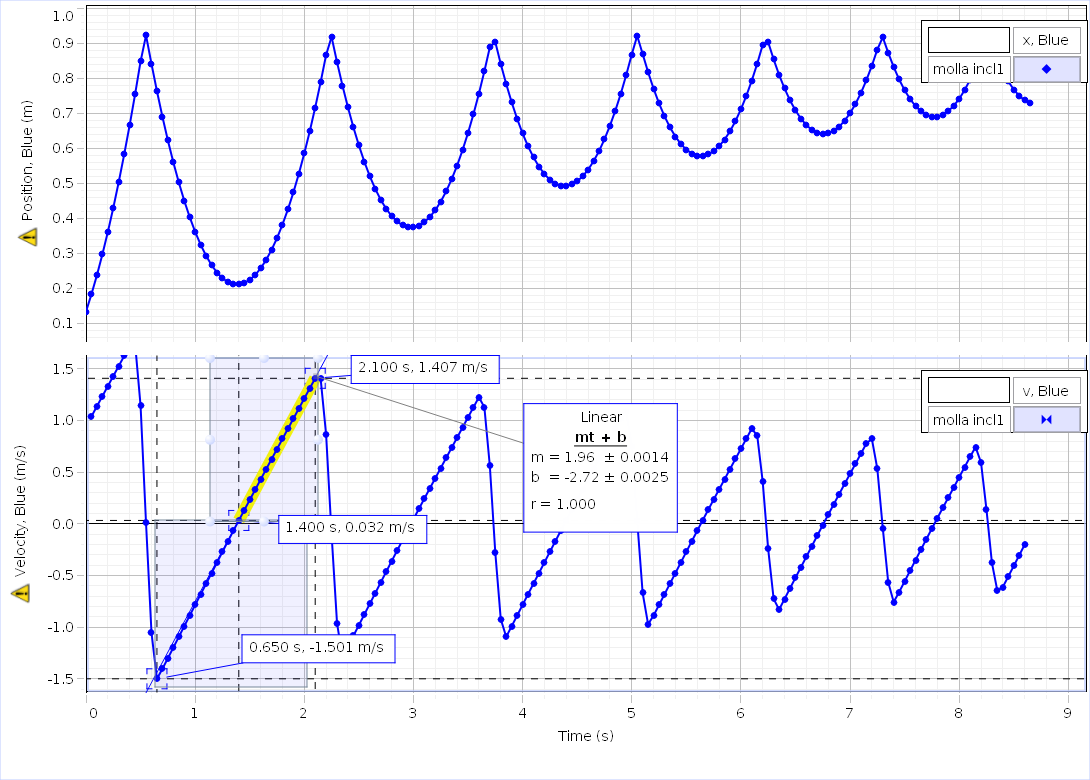
\includegraphics[scale=0.45]{capstone_data/attrito1.png}
				\caption{discesa: coefficiente angolare = \(1.96 \pm 0.0014\)}
			\end{subfigure}%
			
			\begin{subfigure}{0.9\textwidth}
				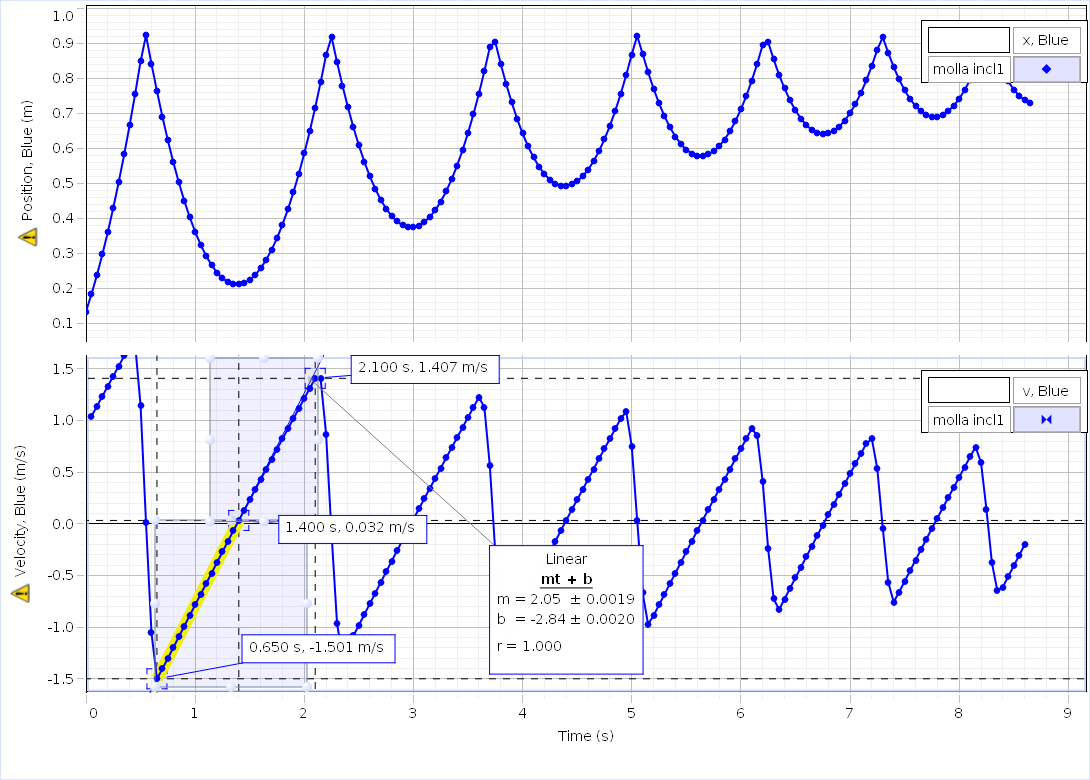
\includegraphics[scale=0.45]{capstone_data/attrito2.png}
				\caption{salita: coefficiente angolare = \(2.05 \pm 0.0019\)}
			\end{subfigure}%
		}
	}
\end{figure}

\begin{figure}[!ht]
	\captionsetup{labelformat=empty}
	\caption{Grafico \(v_{(t)}\) con \(\theta = 12^{\circ}\)}
	\makebox[1 \textwidth][c]{       %centering table
		\resizebox{0.90 \textwidth}{!}{   %resize table
			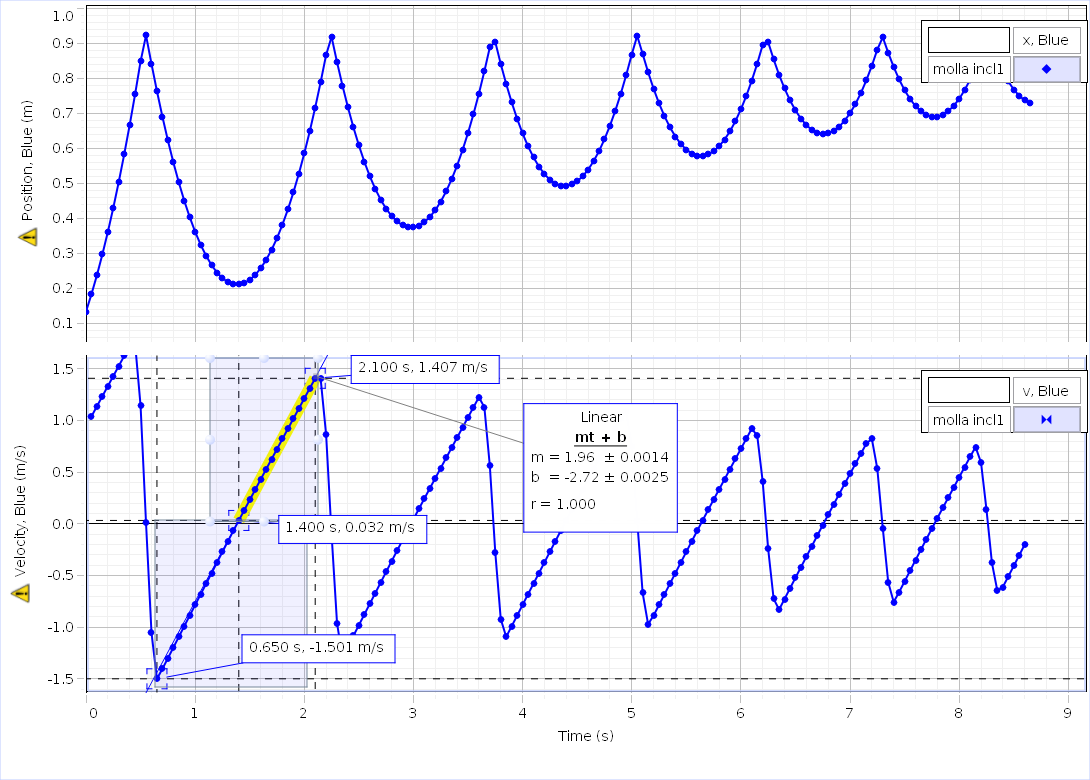
\includegraphics{capstone_data/attrito1.png}
				%\caption{coefficiente angolare=\(1.96 \pm 0.0014\)}
		} %close resize
	} %close centering
	
\end{figure}
			%\caption{coefficiente angolare=\(2.05 \pm 0.0019\)}
\begin{figure}[!ht]
	\captionsetup{labelformat=empty}
	\caption{Grafico \(F_{(x)}\) con due libri davanti al carrello sottoposto a tensione}
	\makebox[1 \textwidth][c]{       %centering table
		\resizebox{0.90 \textwidth}{!}{   %resize table
			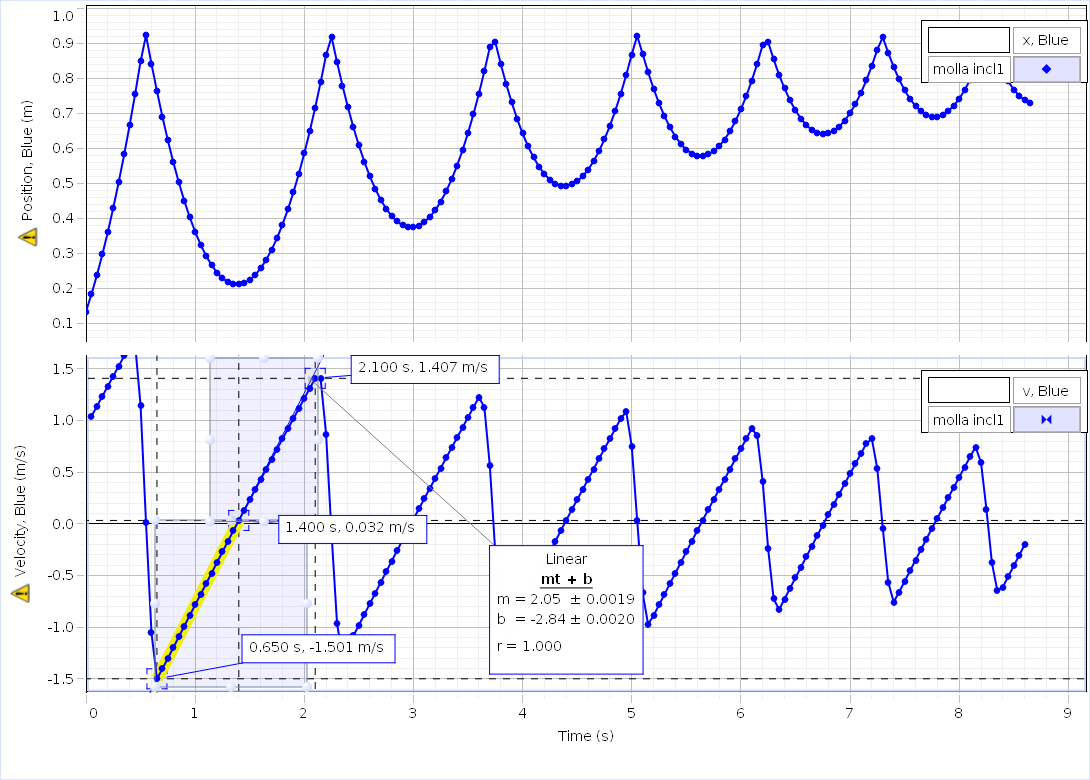
\includegraphics{capstone_data/attrito2.png}

		} %close resize
	} %close centering
	
\end{figure}

\end{document}